% D.30 △ABC（6-8-10 直角）沿 BC 平移 4 单位，重叠四边形
\documentclass[tikz,border=4pt]{standalone}
\usepackage{ctex}
\usepackage{amsmath}
\usetikzlibrary{calc}
\begin{document}
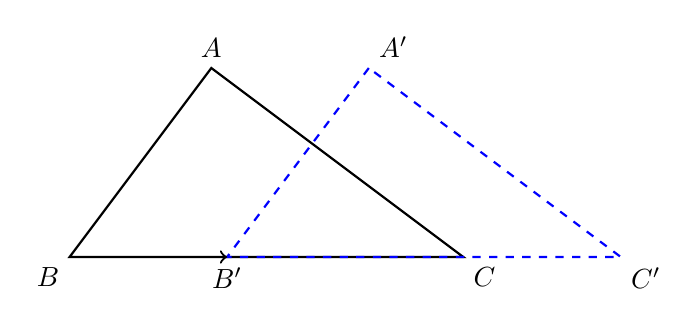
\begin{tikzpicture}[scale=0.5, thick]
  % AB=6, AC=8, BC=10：直角在 A（6²+8²=10²）
  % 取 B=(0,0), C=(10,0), A 使 AB=6,AC=8 → A=(3.6, 4.8)
  \coordinate (B) at (0, 0);
  \coordinate (C) at (10, 0);
  \coordinate (A) at (3.6, 4.8);
  \coordinate (Bp) at (4, 0);
  \coordinate (Cp) at (14, 0);
  \coordinate (Ap) at (7.6, 4.8);

  \fill[orange!20] (Bp) -- (C) -- ($(A)!(C)!(A)$) -- cycle;
  % 重叠四边形：B'、C、(交点)、(交点)
  % 简单画两三角形：
  \draw (A) -- (B) -- (C) -- cycle;
  \draw[blue, dashed] (Ap) -- (Bp) -- (Cp) -- cycle;

  % 平移箭头
  \draw[->, thick] (B) -- (Bp);

  \node[above]       at (A)  {$A$};
  \node[below left]  at (B)  {$B$};
  \node[below right] at (C)  {$C$};
  \node[above right] at (Ap) {$A'$};
  \node[below]       at (Bp) {$B'$};
  \node[below right] at (Cp) {$C'$};
\end{tikzpicture}
\end{document}
